\section{Моделирование термического растекания резиста}


\subsection{Аналитический подход}
Моделирование растекания резиста может быть проведено аналитически на основе подхода, предложенного для моделирования термического растекания периодических структур, полученных в резисте методом НИЛ~\cite{Leveder_2008, Leveder_2011}. В основе этого подхода лежит Фурье-преобразование профиля резиста $h(t)$:
\begin{equation}
	\begin{aligned}
		& h(x, t) = h_0 + \tilde{h}(x, t), \\
		& \tilde{h}(x, t) = \sum_{-\infty}^{+\infty} a_n(t) \exp \left(i n \frac{2 \pi}{\lambda} x\right),
	\end{aligned}
\end{equation}
где $h_0$ -- средняя высота профиля, $\lambda$ -- пространственный период профиля.

Уравнение Навье-Стокса при условии отсутствия проскальзывания и с учетом расклинивающего и Лапласова давления может быть представлено в следующем виде:
\begin{equation} \label{eq:Navier-Stokes}
	\partial_t \tilde{h}-\frac{A}{6 \pi \eta h_0} \partial_x^2 \tilde{h}+\frac{\gamma h_0^3}{3 \eta} \partial_x^4 \tilde{h} = 0,
\end{equation}
где $A$ -- постоянная Гамакера, $\gamma$ -- коэффициент поверхностного натяжения резиста, $\eta$ -- вязкость резиста. Решение уравнения~\ref{eq:Navier-Stokes} приводит к выражению для времени затухания $n$-й пространственной гармоники профиля ($\tau_n$):
\begin{equation}
	\frac{1}{\tau_n}=\left(n \frac{2 \pi}{\lambda}\right)^2 \frac{A}{6 \pi h_0 \eta}+\left(n \frac{2 \pi}{\lambda}\right)^4 \frac{\gamma h_0^3}{3 \eta}.
\end{equation}
При выполнении условия $\left(\frac{\displaystyle h_0^2}{\displaystyle \lambda}\right)^2 \ll \frac{\displaystyle A}{\displaystyle \gamma}$ выражение для $\tau_n$ принимает более простой вид:
\begin{equation}
	\tau_n=\frac{3 \eta}{\gamma h_0^3} \times\left(\frac{\lambda}{2 \pi n}\right)^4.
\end{equation}
Результирующий профиль в момент времени $t$ определяется суммой гармоник (рисунок~\ref{fig:ferlow_analytical}):
\begin{equation}
	\tilde{h}(x, t)=\sum_{-\infty}^{+\infty} a_n(0) \exp \left(-\frac{t}{\tau_n}+i n \frac{2 \pi}{\lambda} x\right).
\end{equation}

\begin{figure}
	\begin{center}
		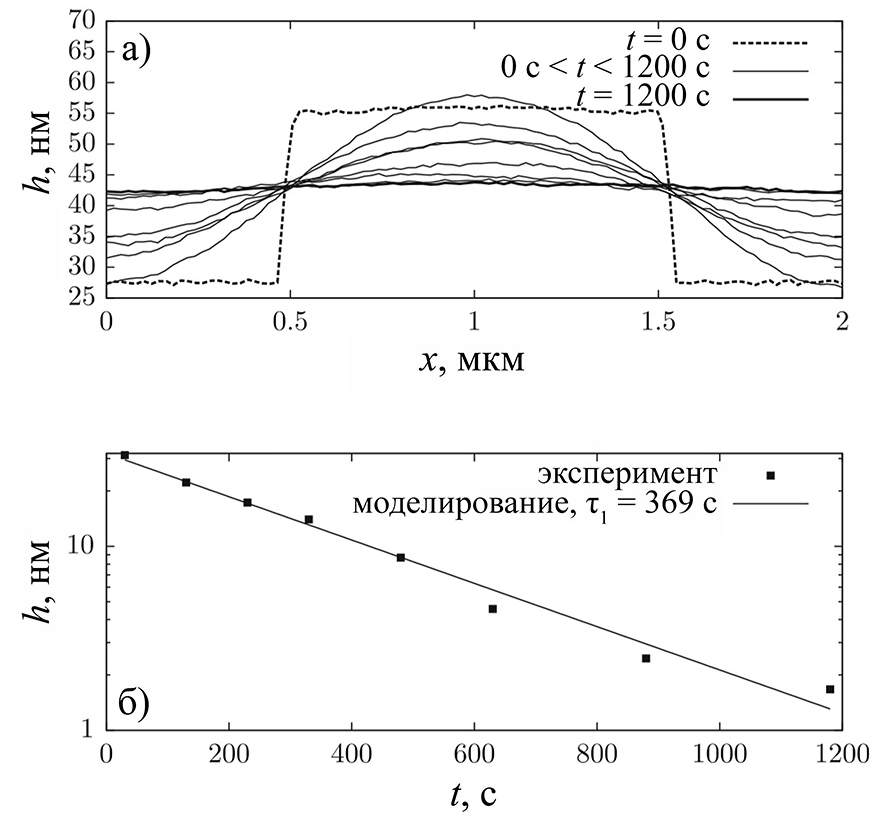
\includegraphics[width=0.7\linewidth]{jpg/reflow_Leveder_large_200}
		\caption{Растекание решетки с периодом 2 мкм, полученной в ПММА методом наноимпринтной литографии~\cite{Leveder_2011}. Нагрев производился при температуре 145~$^\circ$С, время нагрева составляло от 50 до 1200 с: а) 2D профили, полученные методом атомно-силовой микроскопии, б) зависимость высоты профиля решетки от времени в эксперименте (точки) и при моделировании со значением $\tau_1$ = 369 c (сплошная линия).}
		\label{fig:ferlow_analytical}
	\end{center}
\end{figure}

Следует отметить, что вязкость резиста зависит как от температуры резиста, так и от его молекулярной массы. Температурная зависимость вязкости резиста может быть описана уравнением Вильямса-Ландела-Ферри~\cite{bird1987dynamics_WLF}:
\begin{equation} \label{eq:WLF}
	\log \left( \frac{\eta(T)}{\eta(T_0)} \right) = -\frac{C_1(T-T_0)}{C_2+(T-T_0)},
\end{equation}
где $T$ -- температура резиста, значения $\eta(T_0)$, $C_1$, $C_2$ и $T_0$ для различных резистов приведены в таблице~\ref{table:WLF}~\cite{aho2008measurement_WLF}.

Зависимость вязкости резиста от его молекулярной массы может быть описана эмпирической формулой:
\begin{equation} \label{eq:3p4_3p1}
	\eta \propto \Mn^\alpha,
\end{equation}
где $\Mn$ -- среднечисловая молекулярная масса резиста, значение параметра $\alpha$ для ПММА составляет 3.4 при $\Mn$ $\geq$ 48000 и 1.4 при $\Mn$ $<$ 48000~\cite{Leveder_2010, Bueche_3p4_1p4}.

\begin{table}[h]
	\centering
	\caption{Значения параметров функции~\ref{eq:WLF} для полистирола (ПС), полиметилметакрилата (ПММА) и поликарбоната (ПК)~\cite{aho2008measurement_WLF}.}
	\begin{tabular}{l c c c}
		\hline \hline \\ [-1em]
		Параметр \hspace{2em} & ПС \hspace{2em} & ПММА \hspace{2em} & ПК
		\\ \hline \\ [-1em]
		$\eta(T_0)$, Па с \hspace{2em} & 7310.4 \hspace{2em} & 13450 \hspace{2em} & 2763
		\\ \\ [-1em]
		$C_1$ \hspace{2em} & 10.768 \hspace{2em} & 7.6682 \hspace{2em} & 4.7501
		\\ \\ [-1em]
		$C_2$, $^\circ$C \hspace{2em} & 289.21 \hspace{2em} & 210.76 \hspace{2em} & 110.12
		\\ \\ [-1em]
		$T_0$, $^\circ$C \hspace{2em} & 190 \hspace{2em} & 200 \hspace{2em} & 200
		\\ \hline \hline
	\end{tabular}
\label{table:WLF}
\end{table}


\subsection{Численный подход}
Второй подход к моделированию растекания профиля резиста основан на использовании численного метода конечных элементов, реализованном в программе ``Surface Evolver''~\cite{Brakke_SE}. В этом подходе структурные свойства трехмерного объекта задаются свойствами его поверхности, и эволюция формы объекта в различных процессах описываются изменением формы его поверхности. Моделирование эволюции формы объекта проводится путем минимизации полной поверхностной энергии, при этом объем внутри поверхности на протяжении процесса моделирования поддерживается постоянным. В процессе моделирования поверхность объекта разбивается на треугольные площадки -- грани, задаваемыми тремя узлами -- вершинами, которые, в свою очередь, соединяются ориентированными ребрами (рисунок~\ref{fig:SE_12}). Энергия отдельной грани вычисляется по формуле
\begin{equation}
	E_i=\frac{\gamma_i}{2}\left\|\vec{e}_0 \times \vec{e}_1\right\|,
\end{equation}
где $\gamma_i$ -- коэффициент поверхностного натяжения грани с номером $i$. Сила, действующая на вершину $V_0$ (рисунок~\ref{fig:SE_12}), определяется выражением
\begin{equation}
	\vec{F}_{V_0}=\frac{\gamma_i}{2} \cdot \frac{\vec{e}_1 \times\left(\vec{e}_0 \times \vec{e}_1\right)}{\left\|\vec{e}_0 \times \vec{e}_1\right\|}.
\end{equation}

При моделировании растекания двумерных структур в резисте последние представляются в виде фигуры бесконечной протяженности. При этом моделирование проводится для участка фигуры конечной длины с использованием зеркальных граничных условия на краях участка (рисунок~\ref{fig:SE_3}). Таким образом, возникают три возможных типа граней -- грани на границе полимер/вакуум (p), грани на границе полимер/подложка (ps) и боковые (зеркальные) грани (m). Полная энергия поверхности $E_\mathrm{tot}$ вычисляется по формуле
\begin{equation}
	E_\mathrm{tot} = E_\mathrm{p} - (E_\mathrm{ps} + E_\mathrm{m}),
\end{equation}
где 
\begin{equation}
	E_\mathrm{x} = \sum_{i} E_{\mathrm{x},i}, \hspace{0.5em} \mathrm{x} = \mathrm{p}, \mathrm{ps}, \mathrm{m}.
\end{equation}

\begin{figure}
	\begin{minipage}{0.55\textwidth}
		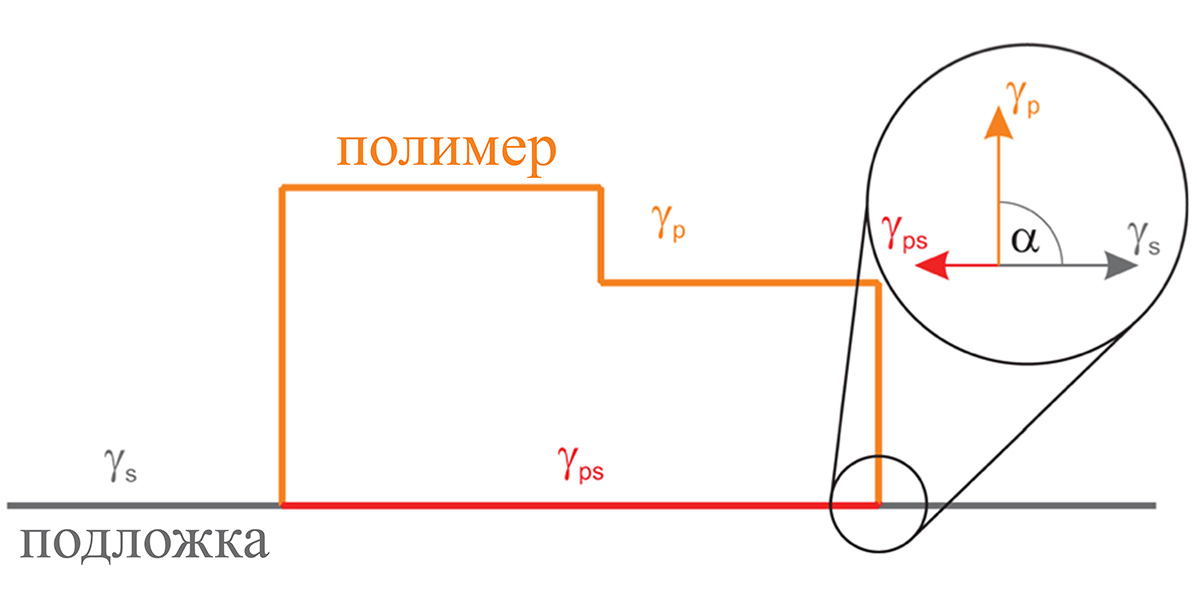
\includegraphics[width=\linewidth]{jpg/SE_1_200}
	\end{minipage}
	\begin{minipage}{0.4\textwidth}
		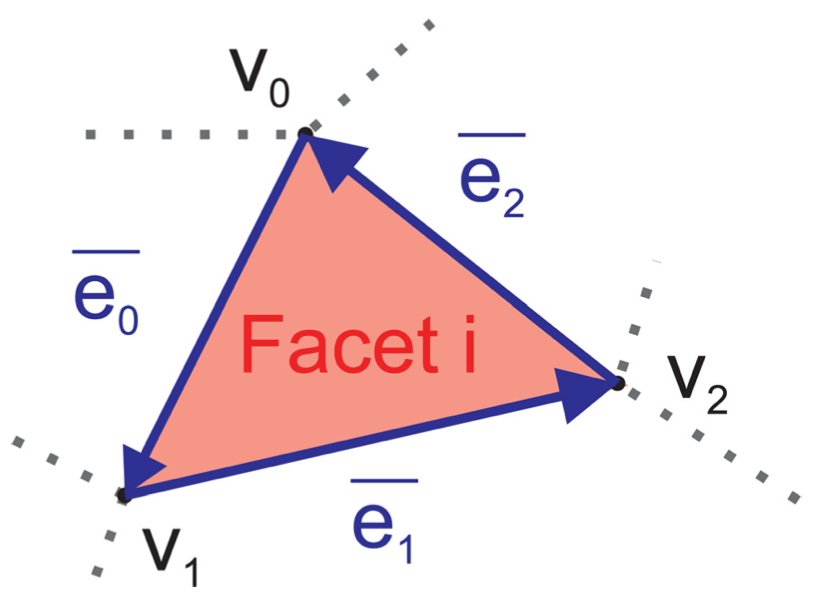
\includegraphics[width=\linewidth]{jpg/SE_2}
	\end{minipage}
	\vspace{0.5em}
	\caption{Схематическое изображение поверхности, заданной в программе ``Surface~Evolver''. $\gamma_\mathrm{p}$, $\gamma_\mathrm{s}$ и $\gamma_\mathrm{ps}$ -- коэффициенты поверхностного натяжения для поверхности полимера, подложки и границы полимер-подложка соответственно, $v_1$, $v_2$ и $v_3$ -- вершины, образующие $i$-ю грань поверхности, $\vec{e_1}$, $\vec{e_2}$ и $\vec{e_3}$ -- ориентированные ребра грани.}
	\label{fig:SE_12}
\end{figure}

В работах по использованию программы ``Surface~Evolver'' для моделирования растекания слоя ПММА моделирование проводилось в режиме нормализации площади, использующемся для реалистичного описания движения под действием сил поверхностного натяжения~\cite{Kirchner_reflow}. В этом режиме при вычислении силы, действующей на вершину, учитывается площадь всех граней, окружающих вершину. Поскольку каждая грань задается тремя вершинами,
сила, действующая на каждую из вершин, будет обратно пропорциональна 1/3 от суммарной площади всех граней, окружающих данную вершину ($A$):
\begin{equation}
	\vec{F}_\mathrm{norm} = \frac{\vec{F}}{A/3} = \frac{3\vec{F}}{A}.
\end{equation}

Связь силы, действующей на вершину, со скоростью движения вершины в процессе моделирования эволюции поверхности описывается коэффициентом подвижности вершины $\mu$:
\begin{equation} \label{eq:SE_v}
	\vec{v} = \vec{F}_\mathrm{norm} \cdot \mu = \frac{\vec{F}}{A/3} \cdot \mu.
\end{equation}
Смещение вершины определяется формулой
\begin{equation} \label{eq:SE_delta}
	\boldsymbol{\delta} = \vec{v} \cdot s,
\end{equation}
где $s$ -- величина, называющаяся ``scale'' и использующаяся в качестве временной переменной.

Следует отметить, что в исходном виде данный метод применяется только для определения конечной формы поверхности, поскольку связь величины $s$ со временем, а также связь подвижности вершин поверхности с физическими величинами, описывающими слой полимера, до настоящего времени не были известны.


\begin{figure}[t]
	\begin{center}
		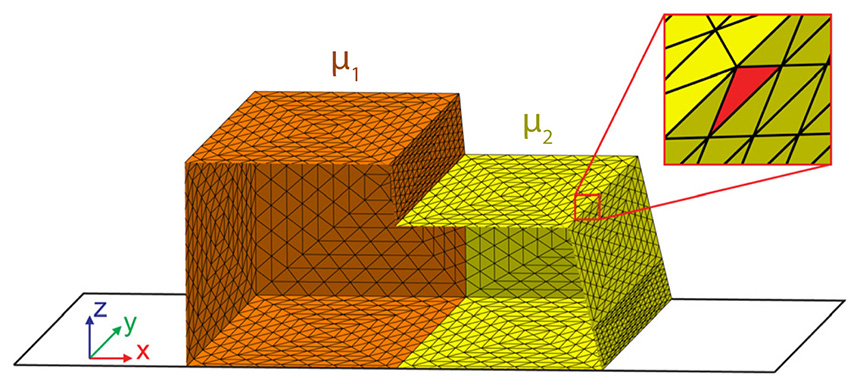
\includegraphics[width=0.9\linewidth]{jpg/SE_3_medium}
		\vspace{1em}
		\caption{Модель поверхности образца, полученного методом полутоновой литографии, заданная в программе ``Surface Evolver''~\cite{Kirchner_reflow}. Поверхность состоит из двух частей с различными значениями подвижности вершин ($\mu_1$ и $\mu_2$).}
		\label{fig:SE_3}
	\end{center}
\end{figure}
